\paragraph{}
In this section we will make a quick review of all the models we passed through trying to illustrate its architecture ,its performance and all the problems we face in each one and how we adapt with it .
\subsection{CNN Model}
As we Mention before in the Review Section ,we follow \textbf{Facial Expression Recognition using Convolutional Neural Networks: State of the Art} Paper\cite{state_of_art} model numebr Five .
on \textbf{fer13} dataset this model follow this Paper \textbf{Learning Social Relation Traits from Face Images} this model Architecture is \textbf{CPNCPNCPCFF} \footnote{ the operations C , P ,N ,F denote to covolutional ,Pooling ,Normalization,Fully Connected }, we get the accuracy mentioned in tabel \ref{tab:14model}
\begin{table}[h!]
	\begin{center}
		\caption{Tabel of developing Accuracy throw  5 epoches with Batch size 128 and adeleta optimizer.}
		\label{tab:14model}
		\begin{tabular}{l|c|l|c}
			\textbf{Epoch Number} & \textbf{Training Accuracy} & \textbf{Testing Accuracy} &\textbf{Loss}\\ 
			\hline 
			Epoch 1 & 22.08\% & 13.10\% & 3.6658 \\
			Epoch 2 & 22.23\% & 27.96\% & 3.5919 \\
			Epoch 3 & 23.63\% & 18.54\% & 3.7231 \\
			Epoch 4 & 23.10\% & 27.96\% & 3.4896 \\
			Epoch 5 & 24.42\% & 22.89\% &  3.4968 \\									
			\end{tabular}
	\end{center}

\end{table}
\paragraph{Testing accross Multiple Optimizers}
Over a thousand of both training and testing samples and six epoches we get this final values in table \ref{tab:optimizers}

\paragraph{}
we notice after training this model more and more epoches that this model fall in \textbf{Overfitting problem} ,we found that no matter how many epoches we run the model at certain point the testing accuracy be constant and the training accuracy grow and grow without stopping.and we notice also the model is unstable having un reasonable change in accuracy . 
\begin{table}[h!]
	\begin{center}
		\caption{Tabel of developing Accuracy with respect to different Optimizers with learning rate 0.01 \newline}
		\label{tab:optimizers}
		\begin{tabular}{l|c|l}
			\textbf{Optimizer} & \textbf{Training Accuracy} & \textbf{Testing Accuracy}\\ 
			\hline 
			Adadelta & 38.3\% & 36.3\% \\
			Adagrad & 40.2\% & 33\%\\
			Nadam & 36.8\% & 36\% \\
			Adamax & 37.7\% & 32\% \\
		\end{tabular}
	\end{center}
\end{table}
\paragraph{}
Using the the all dataset with adadelta optimizer ,we get a result of 95\% training accuracy and only 33\% testing accuracy.
\subsubsection{OverFitting and model Stablization}
\paragraph{So we try to Solve this problem }
We found some solutions as :
\begin{enumerate}
	\item Update Layers of Model.
	\item Dealing with Dataset Problems.
	\item apply Cross Validation Technique.
\end{enumerate}
\subsection{Update Layers of Model}
here we try to update layers of our model making it more simple get the feature we need from each image as fast as we can and try to make the gap between accuracy of training and testing small to be accepted.
\textbf{Keep on your mind that we working on fer13 dataset that is challanging data set so we have a big problem here.}
\subsubsection{New Structure}
We update our structure to be as in this Figure \ref{arch}
\begin{figure}
	\centering
	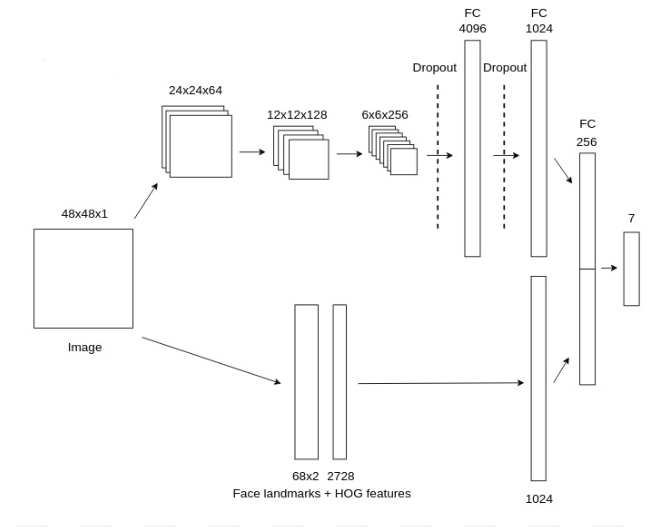
\includegraphics[width=.7\textwidth]{Arch.png}
	\caption{model new Architecture}
	\label{arch}
\end{figure} 
\paragraph{}
We add Hog and Landmark path as a feature extractor methods 
result of this section without Normalization 33\%.
\paragraph{}
After adding Normalization Layers we get \textbf{testing accuracy of 56.93\%} and \textbf{training accuracy of 74\%} after 10 epochs. 
\paragraph{}
We notice an increase now of the accuracy after adding the Normalization layers to this structure.

\subsection{Dealing with datasets problem}
\paragraph{}
one of the data sets we worked was imbalanced "fer13" which made the trained model more biased towards negative emotions (which was more presented in the data set),the solution for this is to balance the data by :
\begin{enumerate}
	\item UnderSampling.
	\item Data Augmentation
\end{enumerate}
\subsubsection{Under Sampling}
\paragraph{results}
Unfortunately this made things even worse with our case since the difference between the size of smallest class and other classes was significant(see Figure~\ref{fig:fer13}) so it results in a large decrease in data set size so a large decrease in learning. \newline

table \ref{tab:table1} shows the how the prediction accuracy of model changes during training epochs, as the table shows, by more training the training accuracy increases, while testing accuracy actually decreases, so this technique couldn't help solve the Overfitting problem we had with the model before it which stopped at about 50\% testing accuracy before overfitting, it even caused a decrease in accuracy, so this technique wasn't a success in his case. 
\begin{table}[h!]
	\centering
	\caption{this table holds the progress of learning for model after under sampling for data set}
	\label{tab:table1}
	\begin{tabular}{c | c | c | c}
		\textbf{Number of Epochs} & \textbf{Training accuracy} & \textbf{Testing accuracy} & \textbf{Error}\\ \hline 
		10 & 39.33 \% & 37.32 \% & 1.69 \\
		20 & 49.08 \% & 36.80 \% & 1.73 \\
		30 & 53.01 \% & 35.64 \% & 1.83 \\
	\end{tabular}
\end{table}

\subsubsection{Data Augmentation}
Also after applying data-augmentation with horizontal-flip as suggested in the paper\cite{state_of_art}
it make things worse in our case .
figure \ref{tab:table12} after more training we find that testing accuracy stop increasing or sometimes start to decrease .
\begin{table}[h!]
	\centering
	\caption{this table holds the progress of learning for model after under sampling for data set}
	\label{tab:table12}
	\begin{tabular}{c | c | c | c}
		\textbf{Number of Epochs} & \textbf{Training accuracy} & \textbf{Testing accuracy} & \textbf{Error}\\ \hline 
		10 & 15.1\% \% & 27\% \% & 1.87 \\
		100 & 20\% \% &  27\%\% & 1.5 \\
	\end{tabular}
\end{table}
\subsubsection{Apply Cross-Validation}
\subsection{Transfer-learning}
\paragraph{}
section \ref{sec:transferlearning} describe what transfer learning is , we choose vgg16 pre trained model to apply it.
\paragraph{VGG16}
is a convolutional neural network model we found it built in layer in keras on imagenet dataset ,so we apply this method with simple dropout and dense layers and it give an accuracy of 27\% for testing .
we find that also vgg16 is not a solution because it suggested that start train this network with at least 1000 sample in each class and we have around 500 sample only in disgust class.
\subsection{Auto-Keras}
\paragraph{}
Autokeras is a new built-in library, tries every possible CNN combination in a period chosen by the user to get the best model structure and configuration.It takes period, training, testing part as an input, its default period is 24 hours and we can get the best model and save it from the program.
After running the code, it stuck in the middle and with online searching about this problem and asking, we found that this is a common problem with this library and it seems to be a bug in it.
